\chapter{考察}
\label{cha:Discussion}

本研究では、既存ツールの有用性の向上を目的として、自然言語仕様書からクラス、操作定義、操作定義を生成する手法を提案した。
さらに、提案手法を既存ツールに適用し、機械学習を活用したVDM++仕様書自動生成ツールVGMLを開発した。
本章では、VGMLに関して考察する。

\section{VGMLの有用性}
本節では、VGMLが自然言語仕様書から自動生成したVDM++仕様書を、人手により記述したVDM++仕様書を正解の仕様書とし、この2つを比較して評価する。
仕様書Aから記述したVDM++仕様書を図\ref{fig:speA_vdm1}-図\ref{fig:speA_vdm6}に、
仕様書Bから記述したVDM++仕様書を図\ref{fig:speB_vdm1}-図\ref{fig:speB_vdm7}に、それぞれ示す。
仕様書Aから人手によって記述したVDM++仕様書は、「intern.vdmpp」、「インターンシップ.vdmpp」、「学生.vdmpp」、「企業.vdmpp」、「企業担当者.vdmpp」、「教員.vdmpp」の6つのファイルから成り、
仕様書Bから人手によって記述したVDM++仕様書は、「advance.vdmpp」、「サークル.vdmpp」、「コース.vdmpp」、「タイム.vdmpp」、「ブロック.vdmpp」、「数字カード.vdmpp」、「走行体.vdmpp」の7つのファイルから成る。

VDM++仕様書は、以下の条件に基づいて記述した。

\begin{itemize}
    \item 自然言語仕様書内の単語の中から、属性や振る舞いなどの情報を持つ可能性があり、かつ、システムの外部に位置するアクターにはなりえない単語を、クラスとして定義する。
    \item 自然言語仕様書内の単語の中から、数字などの不変の情報を持つと判断できる単語を定数名とし、当該単語が持つと判断できる数字などの不変の情報を値として定義する。
    \item 自然言語仕様書内の単語の中から、クラスが持つ属性である可能性がある単語をインスタンス変数定義として定義する。
    \item 自然言語仕様書内の単語の中から、クラスが持つ振る舞いであり、かつ、インスタンス変数を参照する振る舞いである可能性がある単語を操作定義として定義する。
\end{itemize}

今回は、VGMLの有用性の評価のために、VGMLが生成したVDM++仕様書内の単語と、人手で記述したVDM++仕様書内の単語についてのF値\cite{F_value}を測定した。
F値は、適合率と再現率の調和平均である。F値の計算式を、以下に示す。

\begin{equation}
    \mbox F値=\frac{2 \times 適合率 \times 再現率}{適合率+再現率}
\end{equation}	

評価する項目を、以下に示す。

\begin{itemize}
    \item クラスに対する評価
    \item インスタンス変数定義に対する評価
    \item 操作定義に対する評価
\end{itemize}

以降、それぞれの評価について示す。

\subsection{クラスに対する評価}
VGMLが生成するVDM++仕様書におけるクラスと、人手で記述した正解のVDM++仕様書におけるクラスを比較し、一致したクラスをF値を用いて評価する。
クラスに対する評価の適合率は、VGMLが生成したクラスのうち、正解のVDM++仕様書のクラスと一致したクラスの数との割合であり、
再現率は正解のVDM++仕様書のクラスのうち、VGMLが生成したクラスと一致したクラスの数との割合である。
以下に、クラスに対する評価の適合率と再現率の計算式を、それぞれ示す。

\begin{equation}
    \mbox 適合率=\frac{正解の\mathrm{VDM\!+\!+}仕様書のクラスと一致したクラスの数}{VGMLが出力したクラスの数}
\end{equation}
\begin{equation}
    \mbox 再現率=\frac{正解の\mathrm{VDM\!+\!+}仕様書のクラスと一致したクラスの数}{正解の\mathrm{VDM\!+\!+}仕様書のクラスの数}
\end{equation}

VGMLが生成したVDM++仕様書におけるクラスと、正解のVDM++仕様書におけるクラスを比較した際の実験結果を、表\ref{table:classResult}に示す。

表\ref{table:classResult}より、VGMLは、抽出した単語をクラスとして出力する際に、仕様書AでF値1.0、仕様書BでF値0.72の精度で出力できた。
このことにより、VGMLは、教師データと同じ自然言語仕様書において高い割合でクラスを生成できることがわかる。
さらに、教師データの自然言語仕様書と異なる自然言語仕様書に対しても、一定の割合でVDM++仕様書におけるクラスを生成できることがわかる。
よって、VGMLは、既存ツールが生成できる型・定数定義に加え、クラスを記述したVDM++仕様書を一定の割合で生成できるといえる。

VGMLが生成したクラスについて、定性的な評価を述べる。
VGMLは、仕様書Bを基に人手によって記述した正解のVDM++仕様書のクラスの中で、「タイム」と「数字カード」のクラスを抽出できなかった。
「タイム」クラスに関して、「タイム」の概念レベルの値は大きく、クラスの候補である単語の特徴を示していたが、TF-IDF値、出現回数、優先値の値が小さく、
VDM++仕様書に必要でない単語の特徴を大きく示していた。
そのためVGMLは、「タイム」をUNNECESSARYとして分類した。
「数字カード」クラスに関して、TF-IDF値、優先値、連結回数の値が大きく、VDM++仕様書に必要である単語の特徴を示していたが、
概念レベルの値が小さく、クラスの候補でない単語の特徴を示していた。
そのためVGMLは、「数字カード」をNONCLASSとして分類した。
このことから、今後、クラスとしての特徴を示す新たなパラメータが必要であると考える。

\begin{table}[t]
	\caption{VGMLが生成したVDM++仕様書におけるクラスと正解のVDM++仕様書におけるクラスを比較した際の実験結果}
	\label{table:classResult}
	\begin{center}
        \begin{tabular}{c|c|c|c|c|c|c}
            \hline
            仕様書  & 正解の & 出力した &  & 適合率 & 再現率 & F値  \\
                    & VDM++仕様書 & VDM++仕様書 &  一致した       &        &       &      \\
                    & のクラスの数 & のクラスの数 & クラスの数  &        &       &      \\
            \hline
            仕様書A & 5                             & 5                 & 5                  & 1.0   & 1.0    & 1.0  \\
            \hline
            仕様書B & 6                             & 5                  & 4                  & 0.8   & 0.67   & 0.72 \\
            \hline
        \end{tabular}
    \end{center}
\end{table}

\subsection{インスタンス変数定義に対する評価}
VGMLが生成するVDM++仕様書におけるインスタンス変数定義と、人手で記述した正解のVDM++仕様書におけるインスタンス変数定義を比較し、一致したインスタンス変数定義をF値を用いて評価する。
インスタンス変数定義に対する評価の適合率は、VGMLが生成したインスタンス変数定義のうち、正解のVDM++仕様書のインスタンス変数定義と一致したインスタンス変数定義の数との割合であり、
再現率は正解のVDM++仕様書のインスタンス変数定義のうち、VGMLが生成したインスタンス変数定義と一致したインスタンス変数定義の数との割合である。
以下に、インスタンス変数定義に対する評価の適合率と再現率の計算式を、それぞれ示す。

\begin{equation}
    \mbox 適合率=\frac{正解の\mathrm{VDM\!+\!+}仕様書のインスタンス変数定義と一致したインスタンス変数定義の数}{VGMLが出力したインスタンス変数定義の数}
\end{equation}
\begin{equation}
    \mbox 再現率=\frac{正解の\mathrm{VDM\!+\!+}仕様書のインスタンス変数定義と一致したインスタンス変数定義の数}{正解の\mathrm{VDM\!+\!+}仕様書のインスタンス変数定義の数}
\end{equation}

VGMLが生成したVDM++仕様書におけるインスタンス変数定義と、正解のVDM++仕様書におけるインスタンス変数定義を比較した際の実験結果を、表\ref{table:instanceResult}に示す。

表\ref{table:instanceResult}より、VGMLは、抽出した単語をインスタンス変数定義として出力する際に、仕様書AでF値0.62、仕様書BでF値0.61の精度で出力できた。
このことにより、VGMLは、教師データの自然言語仕様書と同じ自然言語仕様書と、異なる自然言語仕様書に対しても、一定の割合でVDM++仕様書におけるインスタンス変数定義を生成できることがわかる。
よって、VGMLは、既存ツールが生成できる型・定数定義に加え、インスタンス変数定義を記述したVDM++仕様書を一定の割合で生成できるといえる。

VGMLが生成したインスタンス変数定義について、定性的な評価を述べる。
VGMLは、クラスの候補である単語に接続する単語を基にインスタンス変数定義の候補である単語を抽出する。
そのため、クラスの候補である単語に接続しない単語の中からインスタンス変数定義の候補である単語を抽出することができない。
これにより、生成できるインスタンス変数定義の候補である単語が少なく、適合率に比べ再現率が低い結果となった。
このことから、今後、クラスの候補である単語に接続する単語以外の単語からも、インスタンス変数定義の候補である単語を
抽出するアルゴリズムを提案する必要があると考える。

\begin{table}[t]
	\caption{VGMLが生成したVDM++仕様書におけるインスタンス変数定義と正解のVDM++仕様書におけるインスタンス変数定義を比較した際の実験結果}
	\label{table:instanceResult}
	\begin{center}
        \begin{tabular}{c|c|c|c|c|c|c}
            \hline
            仕様書  & 正解の & 出力した &  & 適合率 & 再現率 & F値  \\
                    & VDM++仕様書の & VDM++仕様書の & 一致した  &        &       &      \\
                    & インスタンス & インスタンス & インスタンス  &        &       &      \\
                    & 変数定義の数 & 変数定義の数 & 変数定義の数  &        &       &      \\
            \hline
            仕様書A & 20                             & 9                 & 9                  & 1.0   & 0.45    & 0.62  \\
            \hline
            仕様書B & 26                             & 20                  & 14                  & 0.7   & 0.54   & 0.61 \\
            \hline
        \end{tabular}
    \end{center}
\end{table}

\subsection{操作定義に対する評価}
VGMLが生成するVDM++仕様書における操作定義と、人手で記述した正解のVDM++仕様書における操作定義を比較し、一致した操作定義をF値を用いて評価する。
操作定義に対する評価の適合率は、VGMLが生成した操作定義のうち、正解のVDM++仕様書の操作定義と一致した操作定義の数との割合であり、
再現率は正解のVDM++仕様書の操作定義のうち、VGMLが生成した操作定義と一致した操作定義の数との割合である。
以下に、操作定義に対する評価の適合率と再現率の計算式を、それぞれ示す。

\begin{equation}
    \mbox 適合率=\frac{正解の\mathrm{VDM\!+\!+}仕様書の操作定義と一致した操作定義の数}{VGMLが出力した操作定義の数}
\end{equation}
\begin{equation}
    \mbox 再現率=\frac{正解の\mathrm{VDM\!+\!+}仕様書の操作定義と一致した操作定義の数}{正解の\mathrm{VDM\!+\!+}仕様書の操作定義の数}
\end{equation}

VGMLが生成したVDM++仕様書における操作定義と、正解のVDM++仕様書における操作定義を比較した際の実験結果を、表\ref{table:operateResult}に示す。

表\ref{table:operateResult}より、VGMLは、抽出した単語を操作定義として出力する際に、仕様書AでF値0.68、仕様書BでF値0.54の精度で出力できた。
このことにより、VGMLは、教師データの自然言語仕様書と同じ自然言語仕様書と、異なる自然言語仕様書に対しても、一定の割合でVDM++仕様書における操作定義を生成できることがわかる。
よって、VGMLは、既存ツールが生成できる型・定数定義に加え、操作定義を記述したVDM++仕様書を一定の割合で生成できるといえる。

VGMLが生成した操作定義について、定性的な評価を述べる。
VGMLは、文中にクラスの候補である単語が存在した場合、同じ文中に存在する動詞を全て操作定義として抽出する。
そのため、誤った操作定義の候補である単語を多く抽出してしまい、再現率に比べ適合率が低い結果となった。
このことから、今後、クラスの候補である単語と同じ文中に存在する動詞の中から、さらに厳密な分類を行うための
アルゴリズムを提案する必要があると考える。

以上の実験結果から、VGMLは、既存ツールが生成できる型・定数定義に加え、クラス、インスタンス変数定義、操作定義を記述したVDM++仕様書を
一定の割合で生成できるため、既存ツールから、対応するVDM++の構文を増やせたといえる。
従って、VGMLは、既存ツールの有用性を向上したといえる。

\begin{table}[t]
	\caption{VGMLが生成したVDM++仕様書における操作定義と正解のVDM++仕様書における操作定義を比較した際の実験結果}
	\label{table:operateResult}
	\begin{center}
        \begin{tabular}{c|c|c|c|c|c|c}
            \hline
            仕様書  & 正解の & 出力した &  & 適合率 & 再現率 & F値  \\
                    & VDM++仕様書の & VDM++仕様書の & 一致した  &        &       &      \\
                    & 操作定義の数 & 操作定義の数 & 操作定義の数  &        &       &      \\
            \hline
            仕様書A & 31                             & 37                 & 23                  & 0.63   & 0.74    & 0.68  \\
            \hline
            仕様書B & 16                             & 17                  & 9                  & 0.53   & 0.56   & 0.54 \\
            \hline
        \end{tabular}
    \end{center}
\end{table}

\section{関連研究}
自然言語仕様書からVDM++仕様書を生成する研究として、大森氏らの研究\cite{research1,research2}がある。
この研究では、自然言語仕様書と形式モデルの相互変換をサポートし、対応付けを辞書として管理する辞書ツールを開発することによって、
自然言語仕様書からVDM++仕様書を生成できる\cite{research1}。
辞書ツールに自然言語仕様書内の単語を辞書として登録し、登録した単語を類義語やグループ分けの定義や状態として定義することにより、
自然言語仕様書に含まれる曖昧さをなくすことができる。また、入力となる形式的定義と出力する形式的種別を辞書ツールに登録しておくことで、
VDM++仕様書を生成できる。さらに、辞書ツールを使用した形式仕様の作成から実装までを行うことで形式仕様への変換の手順の改良を提案した\cite{research2}。
これによって、辞書ツールを使用した自然言語仕様書から形式仕様の手順を適用することで発生する問題点と、この手順を適用する際に考慮すべき点が発見できた。
大森氏らが開発した辞書ツールが、自然言語仕様書からVDM++仕様書の作成を支援するツールであること対し、VGMLは、機械学習を用いて自然言語仕様書から
VDM++仕様書を自動で生成できる。さらに、VGMLは、既存ツールの型定義と定数定義に加え、クラス、インスタンス変数定義、操作定義の生成が可能である。

また、英語の自然言語仕様書を入力とし、VDM++仕様書を自動で生成する研究として、Lee氏らの研究がある\cite{research3}。
この研究は、英語の要件ドキュメントから形式仕様記述への変換の自動化を目的として、形式仕様記述と言語技術のアプリケーションを提案した。
このアプリケーションは、適切に構造化されたテキストを使用して、英語の要件から知識ベースに変換する。
知識ベースは、英語の要件ドキュメントから構成する。
また、知識ベースからTLG(Two Level Grammar)に変換する。
さらに、自然言語処理によって英語の自然言語仕様書とTLGの曖昧さを解析し、英語の要件ドキュメントから異なる形式を持つ形式仕様言語を生成できる。
この研究は、単語ごとに意味を解析することによって、英語の自然言語仕様書からVDM++仕様書を自動で生成できる。
しかし、日本語の自然言語仕様書の場合は、文章が単語ごとに分ち書きされていない、かつ、1つの単語だけでは意味を持たない可能性があるため、
日本語の自然言語仕様書にそのまま適用することはできない。
これに対し、VGMLは、日本語の自然言語仕様書を対象として、形態素解析によって自然言語仕様書内の文を分かち書きし、
機械学習によって、分かち書きした単語をUNNECESSARY、NONCLASS、CLASSのいずれかに分類する。
さらに、分類した単語をVDM++の構文に当てはめて出力することによって、VDM++仕様書を自動で生成する。
これは、日本語の仕様書を入力として、VDM++仕様書を自動で生成したという点に関して、本研究が初である。

\section{VGMLの問題点}
本研究で開発したVGMLの問題点を、以下に示す。

\begin{itemize}
	\item 関数定義に対応していない\\VGMLは、VDM++を構成する定義ブロックの1つである関数定義には対応していない。この問題については、形態素解析を用いて本研究で抽出した振る舞いを表す単語を、インスタンス変数の候補である単語と関係するか否かの条件を基に分類することで対応できると考える。
	\item VDM++における制約条件に対応していない\\本研究は、自然言語仕様書からVDM++仕様書を生成することを目的としてる。しかし、VGMLが生成するVDM++仕様書は、VDM++仕様書において重要である事前条件、事後条件、不変条件といった制約条件の記述に対応できていない。この問題については、自然言語仕様書内の「最大」、「未満」、「以内」といった範囲を表す単語を抽出し、制約条件として記述するアルゴリズムを提案する必要がある。
	\item 型・定数定義の候補である単語をクラスの候補となる単語へ分類できていない\\VGMLは、抽出した型・定数定義の候補である単語を、クラスの候補となる単語へ分類できない。この問題については、抽出したクラスの候補である単語を多項ロジスティック回帰分析における目的変数とし、型・定数定義の候補である単語を、機械学習を用いてクラスに分類することで対応できると考える。
	\item VDM++仕様書のreal型以外の型に対応していない\\VGMLは、VDM++における型定義を生成する際に、実数型であるreal型しか出力できない。このため、型についてより厳密な仕様書を生成できない。この問題については、VGMLが生成する数値リスト内の数値の条件を表す表現を、自然言語仕様書内から解析することによって対応できると考える。
	\item 操作定義の振る舞いの詳細について記述できていない\\VGMLは、自然言語仕様書が対象とするシステムにおいて、振る舞いを表す単語を操作定義としてVDM++仕様書に記述できる。しかし、その振る舞いの詳細を記述することはできない。この問題については、まず、操作定義の候補である単語が参照するインスタンス変数定義の候補である単語を形態素解析を用いて抽出する。次に、抽出した単語を、操作定義の引数および出力として記述する。最後に、参照するインスタンス変数に対して行う操作を自然言語仕様書から解析することによって対応できると考える。
\end{itemize}

\begin{figure}[p]
    \begin{center}
    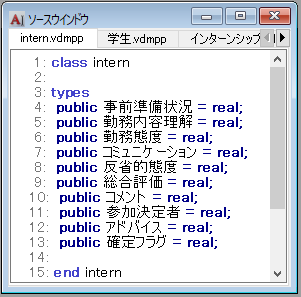
\includegraphics[width=300]{image/speA_vdm1.PNG}
    \caption{仕様書Aから人手によって記述したファイル「intern.vdmpp」}
    \label{fig:speA_vdm1}
    \end{center}
\end{figure}

\begin{figure}[tp]
    \begin{center}
    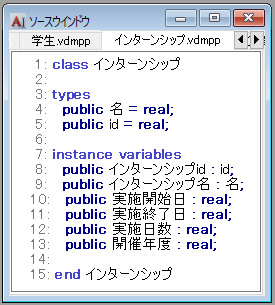
\includegraphics[width=300]{image/speA_vdm2.PNG}
    \caption{仕様書Aから人手によって記述したファイル「インターンシップ.vdmpp」}
    \label{fig:speA_vdm2}
    \end{center}
\end{figure}

\begin{figure}[tp]
    \begin{center}
    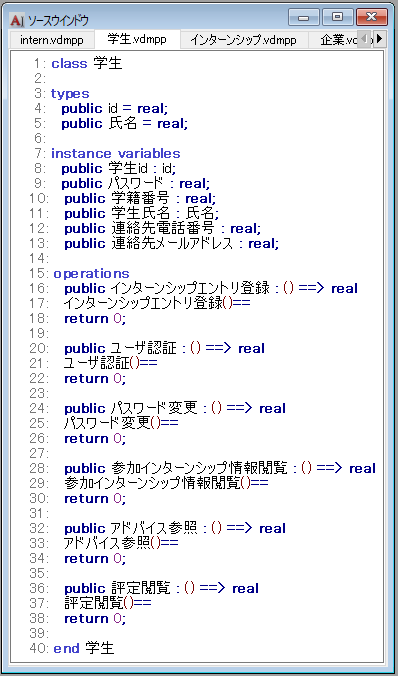
\includegraphics[width=300]{image/speA_vdm3.PNG}
    \caption{仕様書Aから人手によって記述したファイル「学生.vdmpp」}
    \label{fig:speA_vdm3}
    \end{center}
\end{figure}

\begin{figure}[tp]
    \begin{center}
    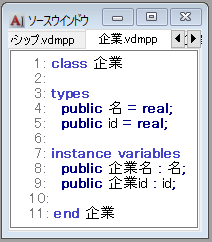
\includegraphics[width=250]{image/speA_vdm4.PNG}
    \caption{仕様書Aから人手によって記述したファイル「企業.vdmpp」}
    \label{fig:speA_vdm4}
    \end{center}
\end{figure}

\begin{figure}[tp]
    \begin{center}
    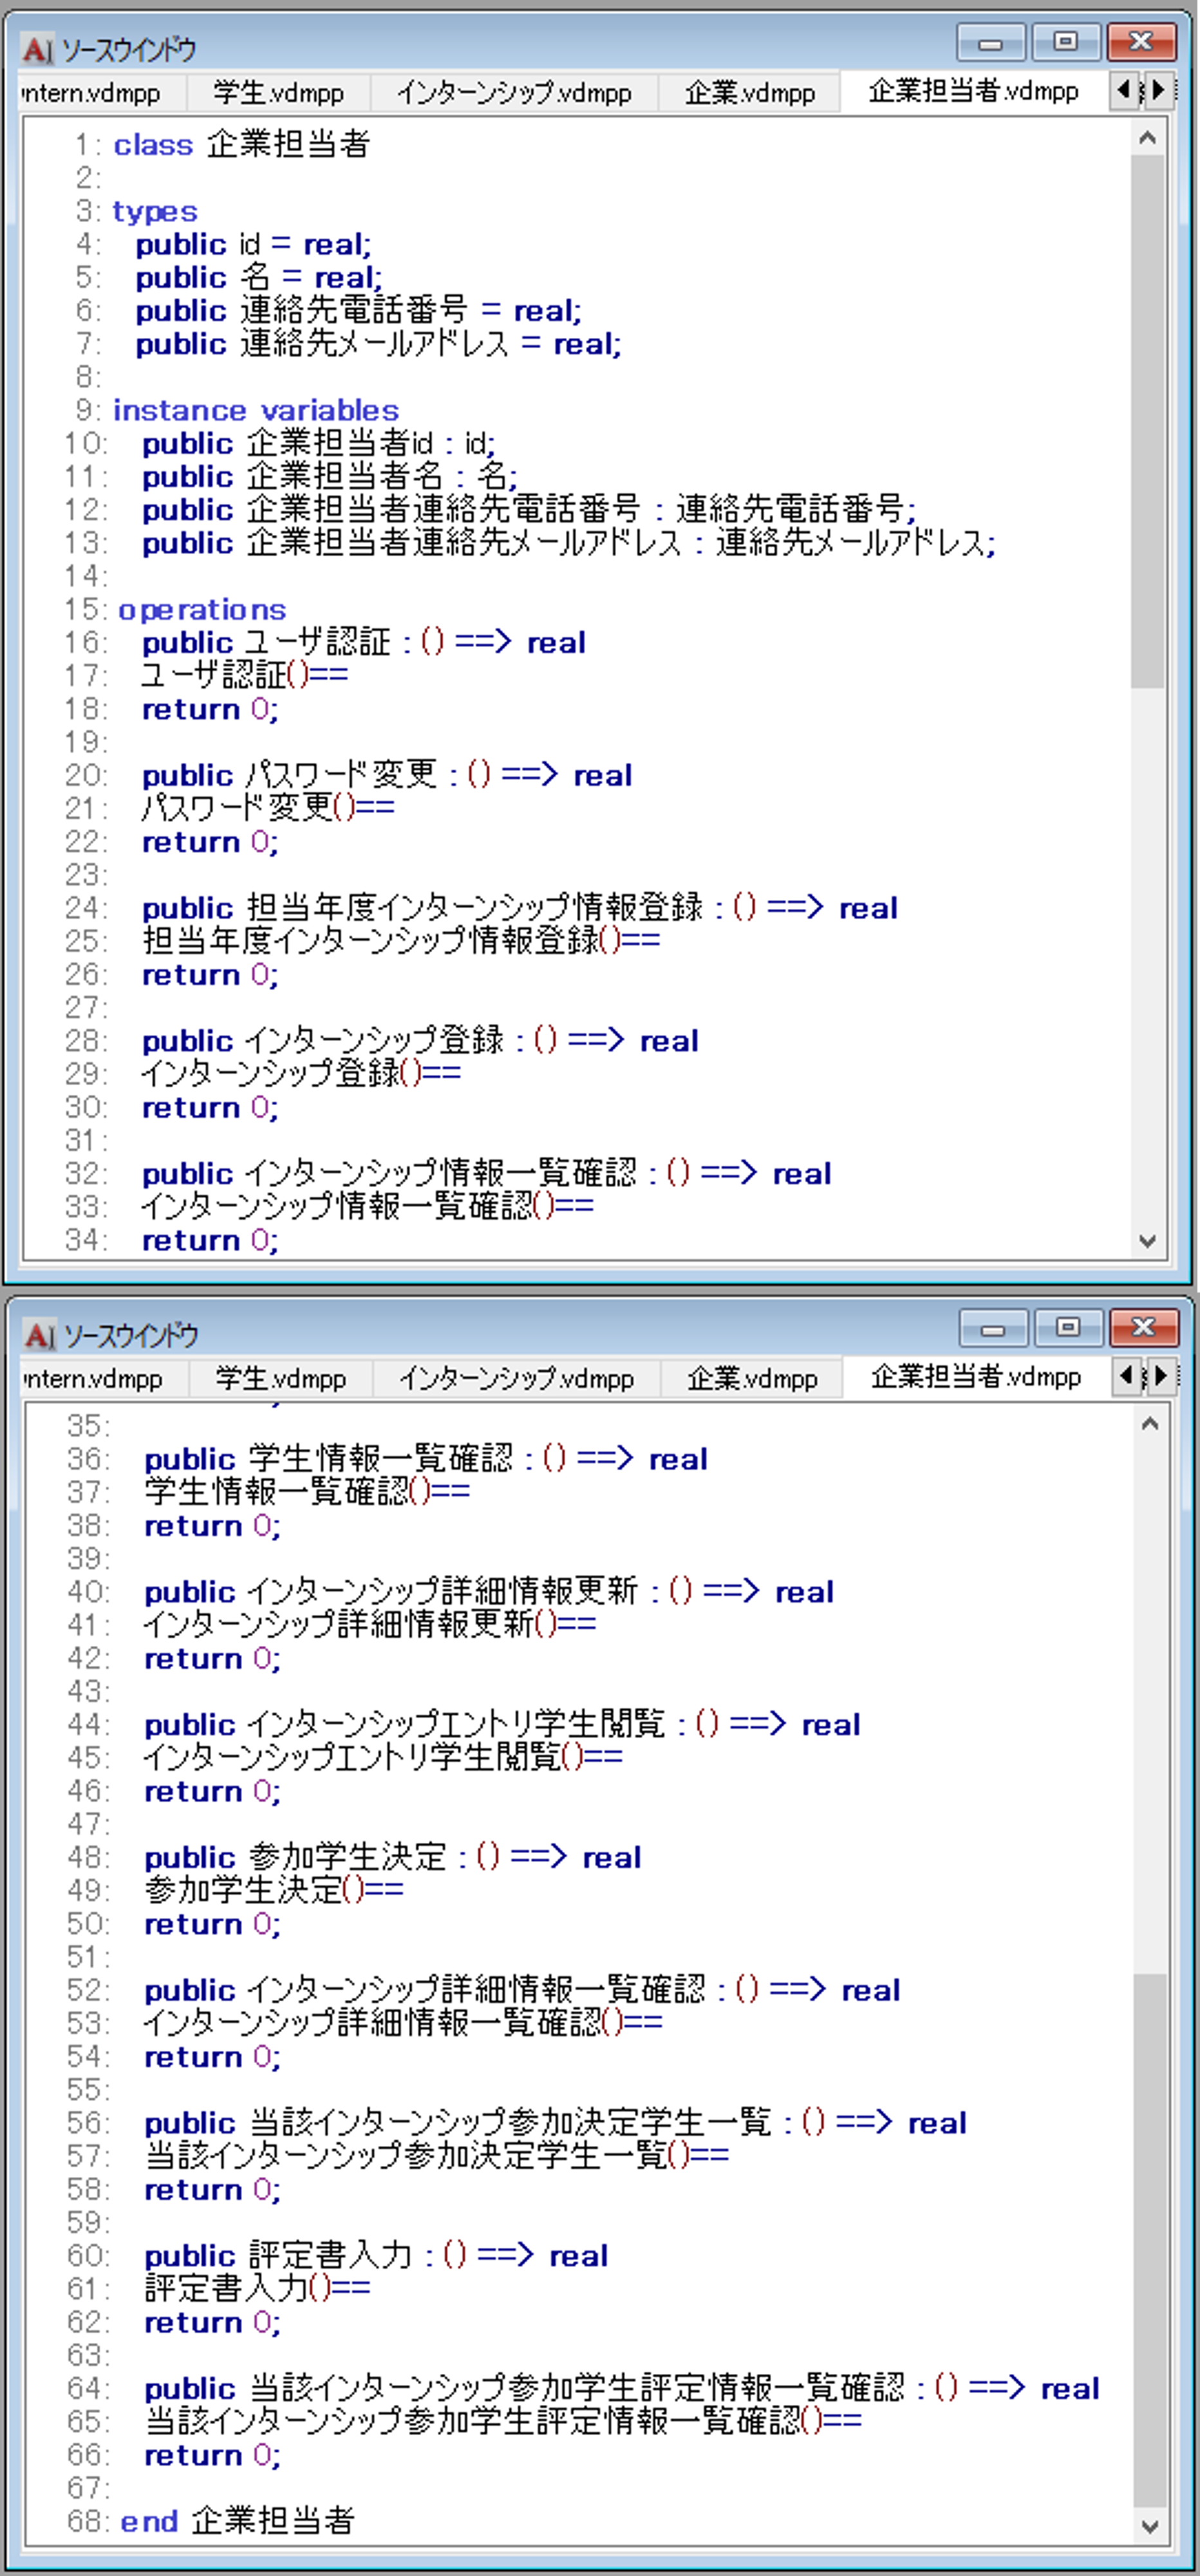
\includegraphics[width=300]{image/speA_vdm5.PNG}
    \caption{仕様書Aから人手によって記述したファイル「企業担当者.vdmpp」}
    \label{fig:speA_vdm5}
    \end{center}
\end{figure}

\begin{figure}[tp]
    \begin{center}
    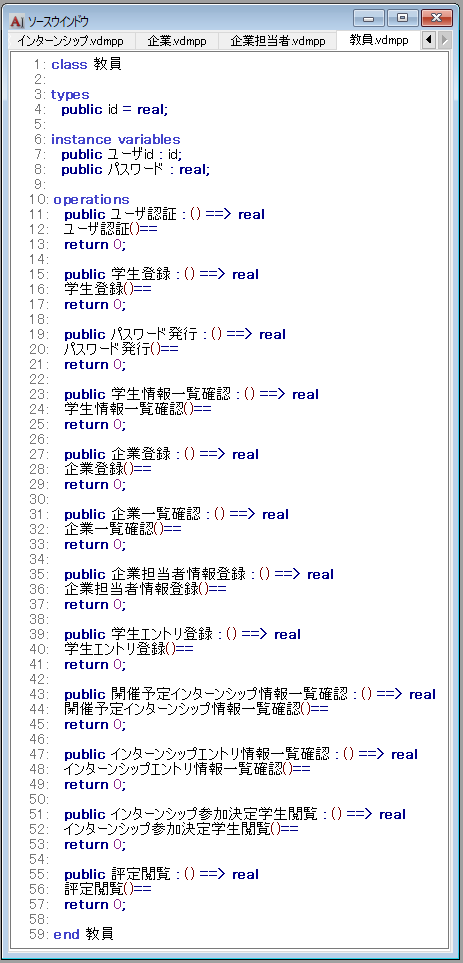
\includegraphics[width=300]{image/speA_vdm6.PNG}
    \caption{仕様書Aから人手によって記述したファイル「教員.vdmpp」}
    \label{fig:speA_vdm6}
    \end{center}
\end{figure}

\begin{figure}[tp]
    \begin{center}
    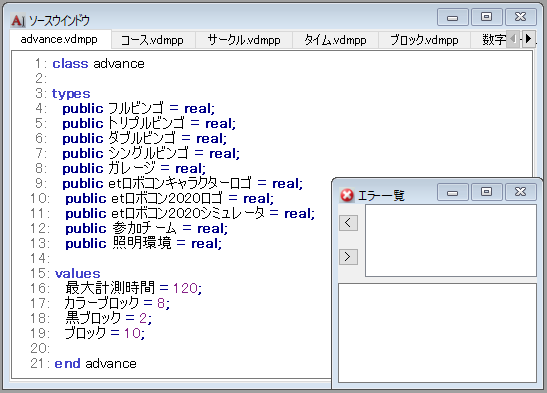
\includegraphics[width=300]{image/speB_vdm1.PNG}
    \caption{仕様書Bから人手によって記述したファイル「advance.vdmpp」}
    \label{fig:speB_vdm1}
    \end{center}
\end{figure}

\begin{figure}[tp]
    \begin{center}
    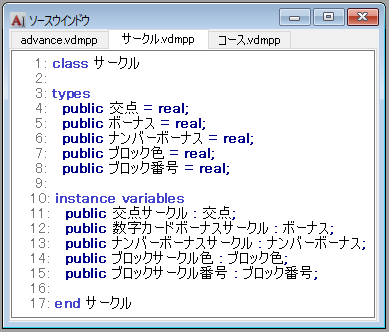
\includegraphics[width=300]{image/speB_vdm2.PNG}
    \caption{仕様書Bから人手によって記述したファイル「サークル.vdmpp」}
    \label{fig:speB_vdm2}
    \end{center}
\end{figure}

\begin{figure}[tp]
    \begin{center}
    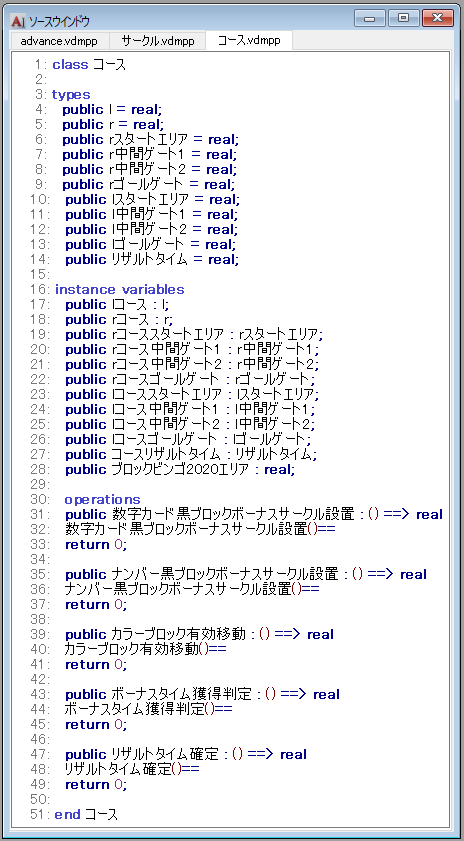
\includegraphics[width=300]{image/speB_vdm3.PNG}
    \caption{仕様書Bから人手によって記述したファイル「コース.vdmpp」}
    \label{fig:speB_vdm3}
    \end{center}
\end{figure}

\begin{figure}[tp]
    \begin{center}
    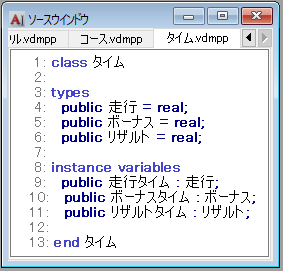
\includegraphics[width=300]{image/speB_vdm4.PNG}
    \caption{仕様書Bから人手によって記述したファイル「タイム.vdmpp」}
    \label{fig:speB_vdm4}
    \end{center}
\end{figure}

\begin{figure}[tp]
    \begin{center}
    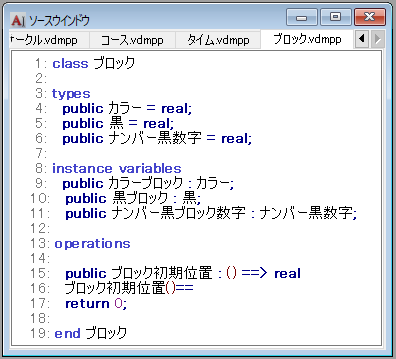
\includegraphics[width=300]{image/speB_vdm5.PNG}
    \caption{仕様書Bから人手によって記述したファイル「ブロック.vdmpp」}
    \label{fig:speB_vdm5}
    \end{center}
\end{figure}

\begin{figure}[tp]
    \begin{center}
    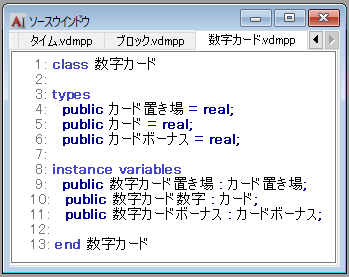
\includegraphics[width=300]{image/speB_vdm6.PNG}
    \caption{仕様書Bから人手によって記述したファイル「数字カード.vdmpp」}
    \label{fig:speB_vdm6}
    \end{center}
\end{figure}

\begin{figure}[tp]
    \begin{center}
    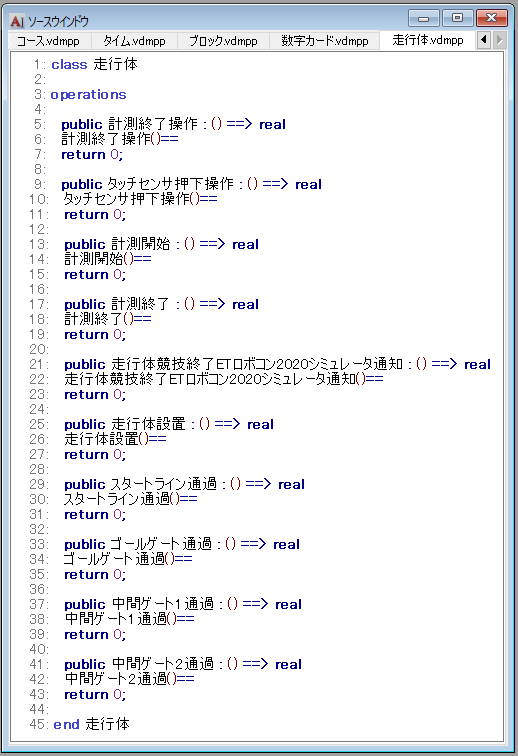
\includegraphics[width=300]{image/speB_vdm7.PNG}
    \caption{仕様書Bから人手によって記述したファイル「走行体.vdmpp」}
    \label{fig:speB_vdm7}
    \end{center}
\end{figure}


